%%%%%%%%%%%%%%%%%%%%%%%%%%%%%%%%%%%%%%%%%%%%%%%%%%%%%%%%%%%%%%%%%%%%%%%%%%%%%%%%
%                              Document Settings                               %
%%%%%%%%%%%%%%%%%%%%%%%%%%%%%%%%%%%%%%%%%%%%%%%%%%%%%%%%%%%%%%%%%%%%%%%%%%%%%%%%

\documentclass[a4paper,12pt]{article}
\usepackage[utf8]{inputenc}
%%%%%%%%%%%%%%%%%%%%%%%%%%%%%%%%%%%%%%%%%%%%%%%%%%%%%%%%%%%%%%%%%%%%%%%%%%%%%%%%
%                                   Margins                                    %
%%%%%%%%%%%%%%%%%%%%%%%%%%%%%%%%%%%%%%%%%%%%%%%%%%%%%%%%%%%%%%%%%%%%%%%%%%%%%%%%

\addtolength{\oddsidemargin}{-1.cm}
\addtolength{\textwidth}{2cm}
\addtolength{\topmargin}{-2cm}
\addtolength{\textheight}{3.5cm}

%%%%%%%%%%%%%%%%%%%%%%%%%%%%%%%%%%%%%%%%%%%%%%%%%%%%%%%%%%%%%%%%%%%%%%%%%%%%%%%%
%                                   Packages                                   %
%%%%%%%%%%%%%%%%%%%%%%%%%%%%%%%%%%%%%%%%%%%%%%%%%%%%%%%%%%%%%%%%%%%%%%%%%%%%%%%%

\usepackage[pdftex]{graphicx}	% Include graphics
\usepackage{float}				% Place floats inline, use the [H] placement
\usepackage{array}				% Additional tables features


%%%%%%%%%%%%%%%%%%%%%%%%%%%%%%%%%%%%%%%%%%%%%%%%%%%%%%%%%%%%%%%%%%%%%%%%%%%%%%%%
%                                   Document                                   %
%%%%%%%%%%%%%%%%%%%%%%%%%%%%%%%%%%%%%%%%%%%%%%%%%%%%%%%%%%%%%%%%%%%%%%%%%%%%%%%%

\begin{document}
	
	% Title page
	% Title page
	\begin{titlepage}
		\begin{center}
			
			% University Logo
			
\includegraphics[width=0.6\textwidth]{../images/up_logo.jpg}\\[2.0cm] 
			
			
			\textsc{\LARGE CS@UP Time Series Prediction}\\[1.0cm]
			
			
			\textsc{\Large User Manual}\\[0.75cm]
			
			
			\textsc{\Large COS301 - Capstone Project}\\[0.75cm]
			
			
			% Students/Contributors Table
			\textbf{\huge \\ Team:}
			\huge NewGen Leaders \\
			\begin{flushright} \large
				Claudio Da Silva		\emph{u14205892} \newline
				Dedr\'e Olwage	    	\emph{u15015239} \newline
				Merrisa Joubert			\emph{u15062440} \newline
				Murray Le Roux	    	\emph{u15311644} \newline
			\end{flushright}
			\small Department of Computer Science, University of Pretoria \\ 
			
			
		\end{center}
		
		% Report Declaration		
		\noindent By submitting this document we confirm that we have read and are aware of the University of Pretoria's policy on academic dishonesty and plagiarism and we declare that the work submitted in this assignment is our own as delimited by the mentioned policies. We explicitly declare that no parts of this assignment have been copied from current or previous students' work or any other sources (including the internet), whether copyrighted or not. We understand that we will be subjected to disciplinary actions should it be found that the work we submit here does not comply with the said policies.
		
		\begin{center}
			
			% Fill page
			\vfill
			
			% Date
			{\large \today}
			
		\end{center}
		
	\end{titlepage}
    
    \tableofcontents
    
    \clearpage
            
    % An overview of the System
    \section{Introduction}
    	
        % Specify the purpose of the product
        \subsection{Purpose}
        
        The purpose of this document is to present a detailed guide on the use of the Time Series Prediction System. It will explain how to setup the system to run in your environment; how to use the system once it is running; as well as deal with frequent errors that may occur during program use. This document is intended for all system users.
          
        % Identify product by name, explain what the product will and will not do, describe the uses of the product including objectives, goals and benefits
        \subsection {Scope}
        
        The system will be used to enter, view, and edit student marks. It will include a prediction system that will use the student marks to make predictions on the outcomes of the students results at the end of the semester. These predictions will be used by lecturers to identify students who need extra help to pass the semester. The predictions may also be used to identify whether the teaching strategies of the lecturer are working as well as they expected it to. The system will allow students to view their marks and it will include an element of gamification that aims to improve student motivation. The ultimate goal of the system is to improve student results. The system also aims to improve the manner in which teaching assistants, tutors and lecturers record marks.
        
        
        \subsection{Definitions,Acronyms and Abbreviations}
        
        \begin{tabular}{ |c|c| } 
        	\hline
        	Term & Definition \\
        	\hline
        	NPM & The Node Package Manager, used to interact with node packages and scripts\\
        	\hline
        \end{tabular}
       
  	\pagebreak
  	
    \section{Installing the software}

    	% Things to note before setting up the system
    	\subsection{Before you begin}
    	
    	Before starting with the system, ensure that the following key features are installed for the various sections:
    	
    	\begin{itemize}
    		\item \textbf{Docker}
    		\begin{itemize}
    			\item Ensure you have version 17 or up of the standard Docker installation
    			\item Ensure you have Docker Compose version 3 installed
    			\item Both can be obtained from the docker website
    		\end{itemize}
    	\end{itemize}
    
    	\begin{itemize}
	    	\item \textbf{Server}
	    	\begin{itemize}
	    		\item Ensure you have NodeJS 6.10 or the latest stable version installed
	    		\item Ensure you have the latest stable release of MongoDB installed
	    		\item Ensure RabbitMQ is properly setup
	    		\item Ensure Python 3 is correctly installed
	    		\item Ensure Tensorflow is correctly installed
	    		\item Node can be obtained from the NodeJS website, MongoDB can be obtained from the mongodb website
	    	\end{itemize}
    	\end{itemize}
    
       	\begin{itemize}
	    	\item \textbf{Client}
	    	\begin{itemize}
    			\item Ensure you have NodeJS 6.10 or the latest stable version installed
    			\item Ensure you have the Angular CLI for Angular2
	    		\item Node can be obtained from the NodeJS website, the angular CLI can be installed by using the command, "npm install -g angular/cli" 
	    	\end{itemize}
    	\end{itemize}
   	
    	% Explains how to setup the system making use of the dockehub image or docker-compose up
    	\subsection{Using a system Docker image}
    	
    		\subsubsection {Retrieving the files}
    		
    		Once a Docker Hub image becomes available we will add the link in here
    		
    		\subsubsection {Compiling and running the software}
    		
   		  	\begin{itemize}
    			\item \textbf{Using Docker Hub}
    			\begin{itemize}
    				\item Once a Docker Hub image becomes available we will add the link in here
    			\end{itemize}
    		\end{itemize}
   		  	\begin{itemize}
    			\item \textbf{Using cloned repository}
    			\begin{itemize}
    				\item Simply enter into the folder you wish to compile. In the same location as the docker-compose.yml, run the following command in terminal, "docker-compose up"
    			\end{itemize}
    		\end{itemize}

    	% Setting up the server as a standalone system for use with another client, either using docker-compose or the manual way
     	\subsection{Server}
     	
	    	\subsubsection {Retrieving the files}
	    	
	    	To obtain the files for the server portion of the application, simply run the command, "git clone https://github.com/TimeSeriesPrediction/time-series-server"
   	    		
	     	\subsubsection {Compiling the software}
	     	
	     	In order to be able to run the server, first enter into the cloned folder. While inside this folder, use a terminal and enter the command, "npm install". This will obtain all the required dependencies in order to run the program.
	     	
	     	\subsubsection {Running the software}
	     	
	     	To run the server, first ensure the configuration file, contained under config called default.json contains the correct information for your system. Once that is done, enter into a terminal within the root of the folder, and run the command, "npm start"
     
       	% Setting up the client as a standalone system for use with another server, either using docker-compose or the manual way
     	\subsection{Client}
     	
     		\subsubsection {Retrieving the files}
     		
     		To obtain the files for the server portion of the application, simply run the command, "git clone https://github.com/TimeSeriesPrediction/time-series-web-client"
     		
     		\subsubsection {Compiling the software}
     				
     		In order to be able to run the client, first enter into the cloned folder. While inside this folder, use a terminal and enter the command, "npm install". This will obtain all the required dependencies in order to run the program.
     		
     		\subsubsection {Running the software}
     		
	     	To run the client, enter into a terminal within the root of the folder, and run the command, "npm start". As an alternative, one can make use of the command, "ng serve"
    
    \pagebreak
    % How to use the various features of the system
    
    \section{Using the software}
    
   		%The feature that involves adding new users to a system, either from a database or using a registration system
    	\subsection{Logging in}
    	
    	When accessing the client, one will be given the option to login. If a user is registered on the system, one needs simply enter the username and password tied to their account to be given access. The user will be automatically logged out within an hour if no activity is recorded from their account. If a user happens to forget their password, they may use the reset password feature.\\[1.0cm]
        
        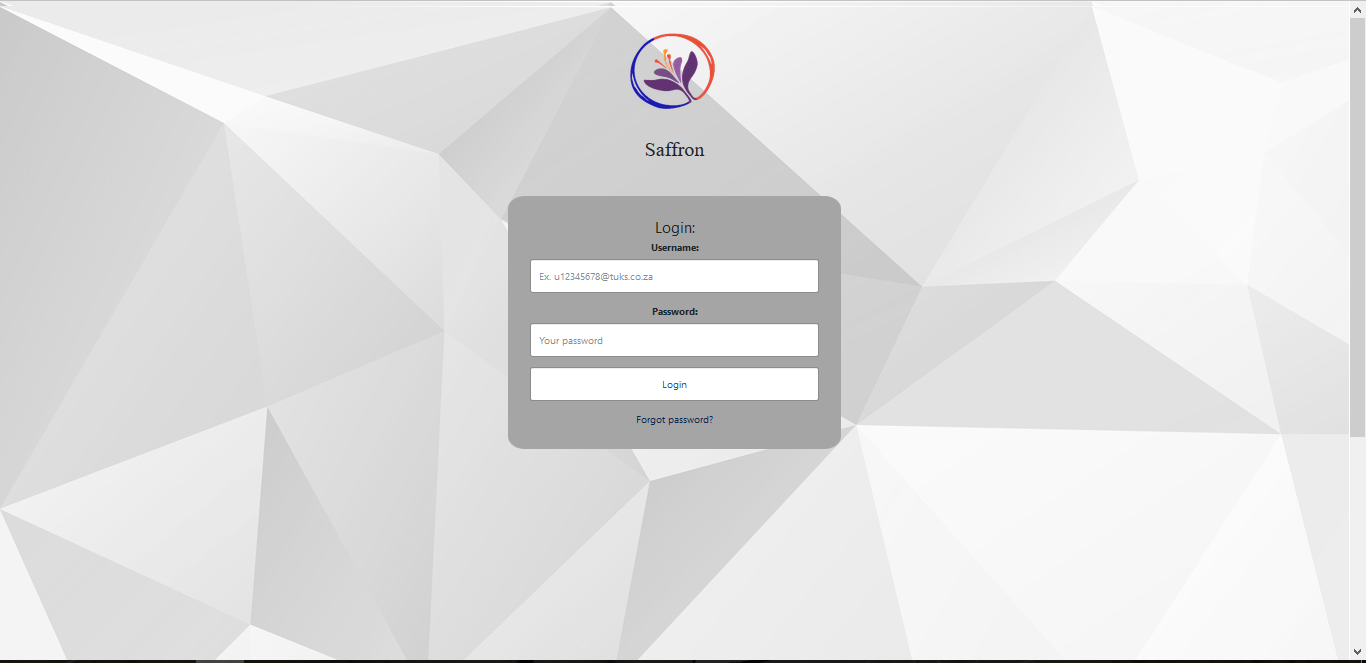
\includegraphics[width=1\textwidth]{../images/screens/login.PNG}\\[1.0cm] 
    	
   		\subsection{Resetting a password}
    	
    	If a user happens to forget their password, they may use the forgot password link available on the login screen. The user will then have an email sent to the email account linked to their username. Once the email is received, the user will have an hour in order to follow the link given in order to enter a new password. Each reset is unique and will only work once.\\[1.0cm]
        
        %\includegraphics[width=1\textwidth]{../images/screens/reset-password.PNG}\\[1.0cm] 
    	
    	\subsection{Adding a new user}
    	
        If a user has the correct permissions, they will have the rights to add new users to the system. New users can be entered in bulk, by uploading a formatted Excel spreadsheet file from their computer. Single new users can also be added through the interface provided.\\[1.0cm]
        
        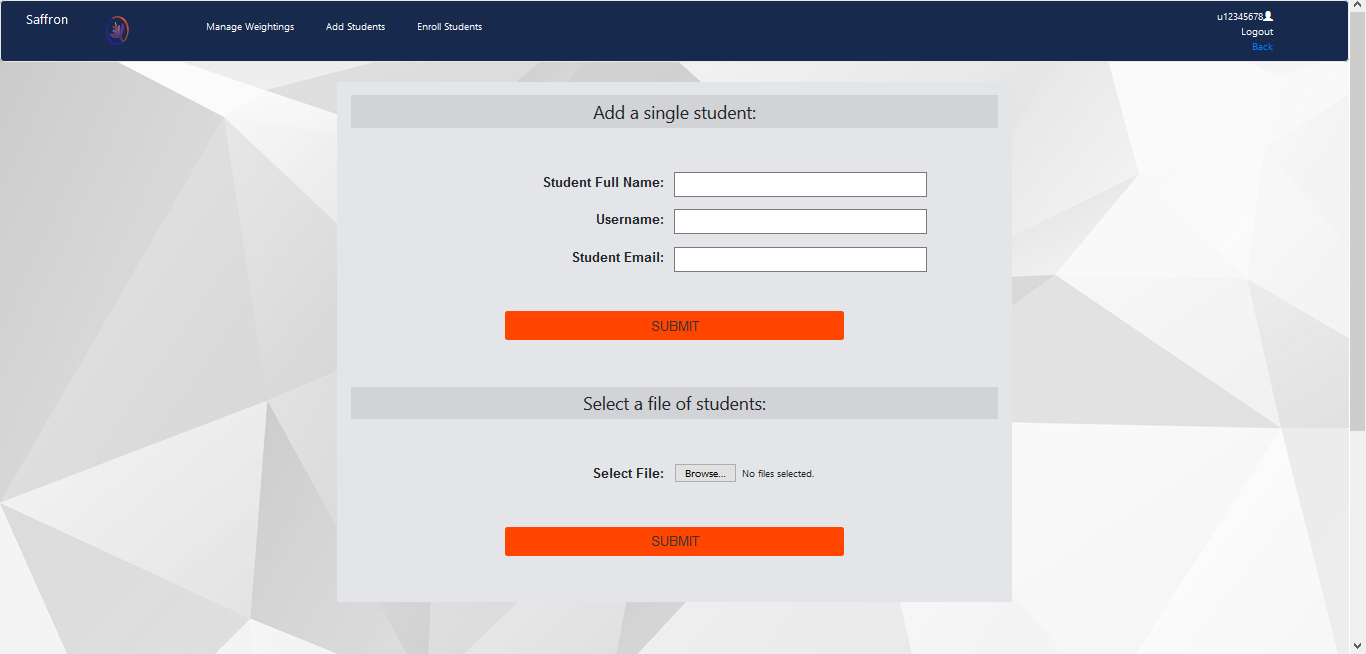
\includegraphics[width=1\textwidth]{../images/screens/add-bulk-students.PNG}\\[1.0cm]  
        
    	\subsection{Adding a new assessment}
        
        If a user has the correct permissions, they have the rights to add different assessments for different modules. This can be done by providing the module code, assessment type etc. to the interface fields.\\[1.0cm]
        
        %\includegraphics[width=1\textwidth]{../images/screens/assignments.PNG}\\[1.0cm]
        
        \subsection{Enrolling students for a module}
        
        If a user has the correct permissions, they have the rights to enroll students to a specific module. Students can be enrolled through uploading an Excel spreadsheet file containing the student numbers of the students to be enrolled for that specific module.\\[1.0cm]
        
        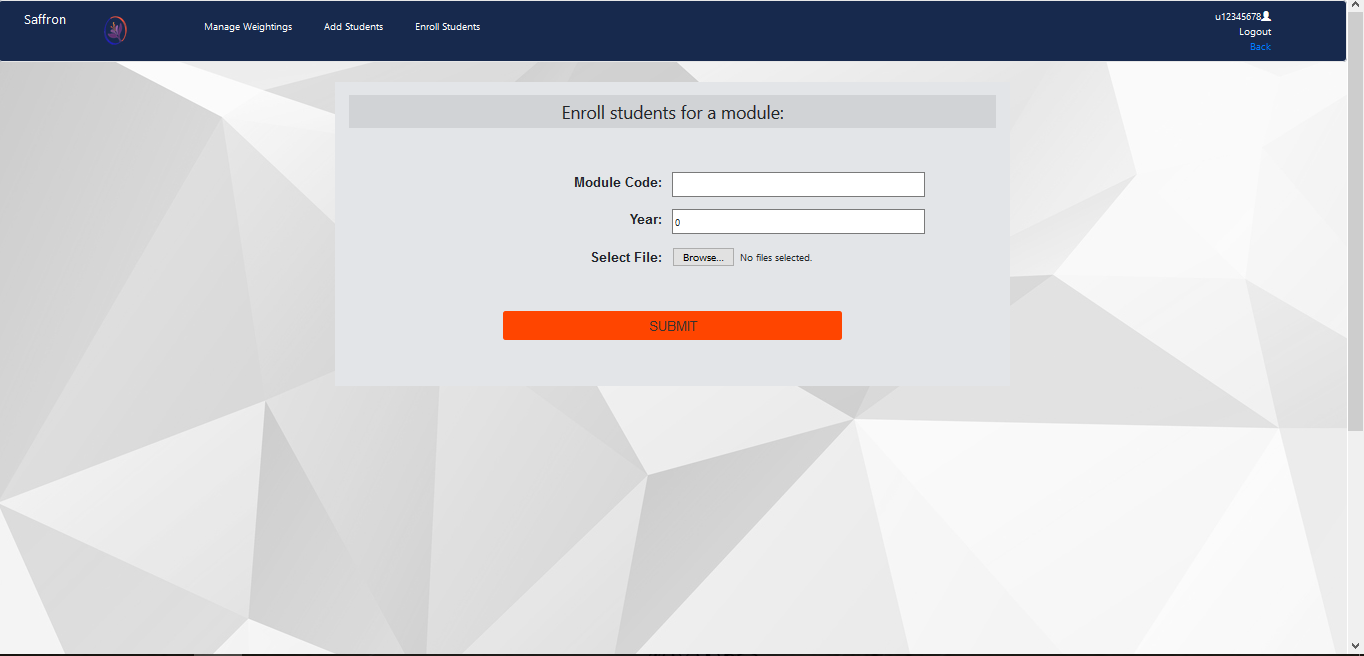
\includegraphics[width=1\textwidth]{../images/screens/enroll-students.PNG}\\[1.0cm]
     	\pagebreak
    	\subsection{View your assessment marks for a module}
        
        A student (or user) can view the marks that they have obtained for a specific assessment (such as a test) by heading over to this interface. On this interface, users are also offered the opportunity to easily query their mark, given that the query time for that mark has not yet expired.\\[1.0cm]
        
        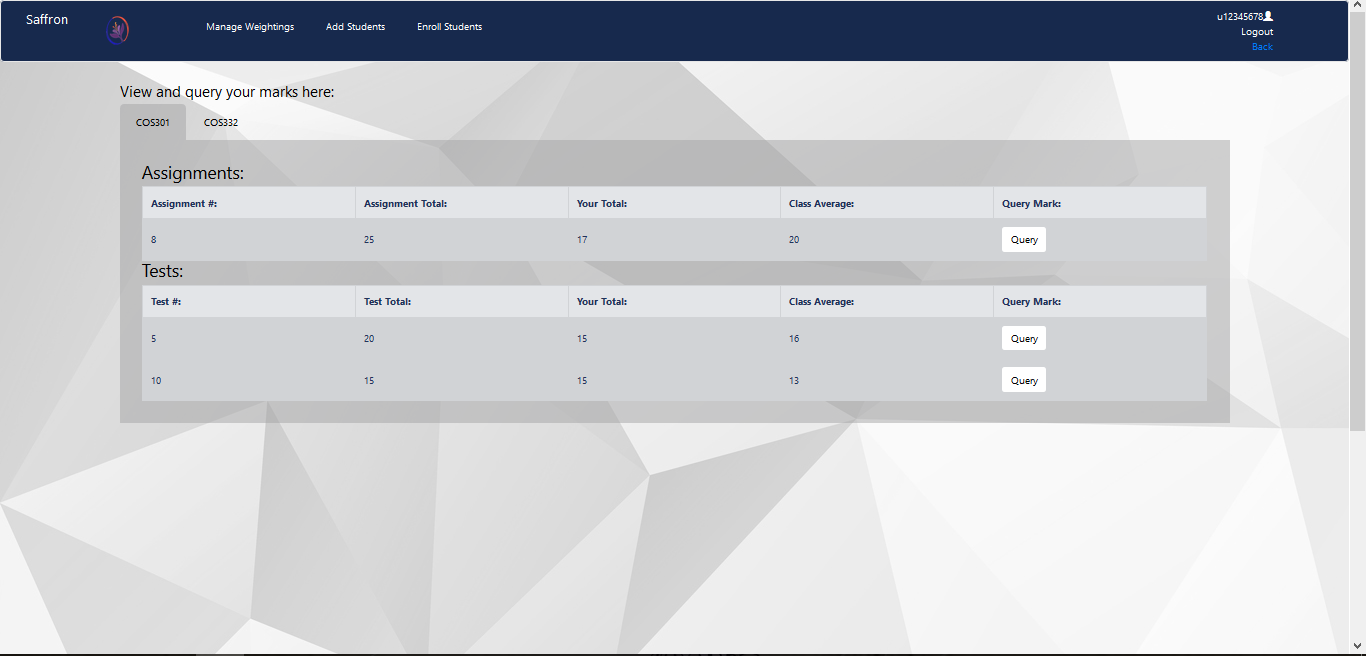
\includegraphics[width=1\textwidth]{../images/screens/student-view-marks.PNG}\\[1.0cm]
        
        \subsection{Add weightings for a module}
        
        If a user has the correct permissions, they have the rights to add weights for a specific module. 
        
        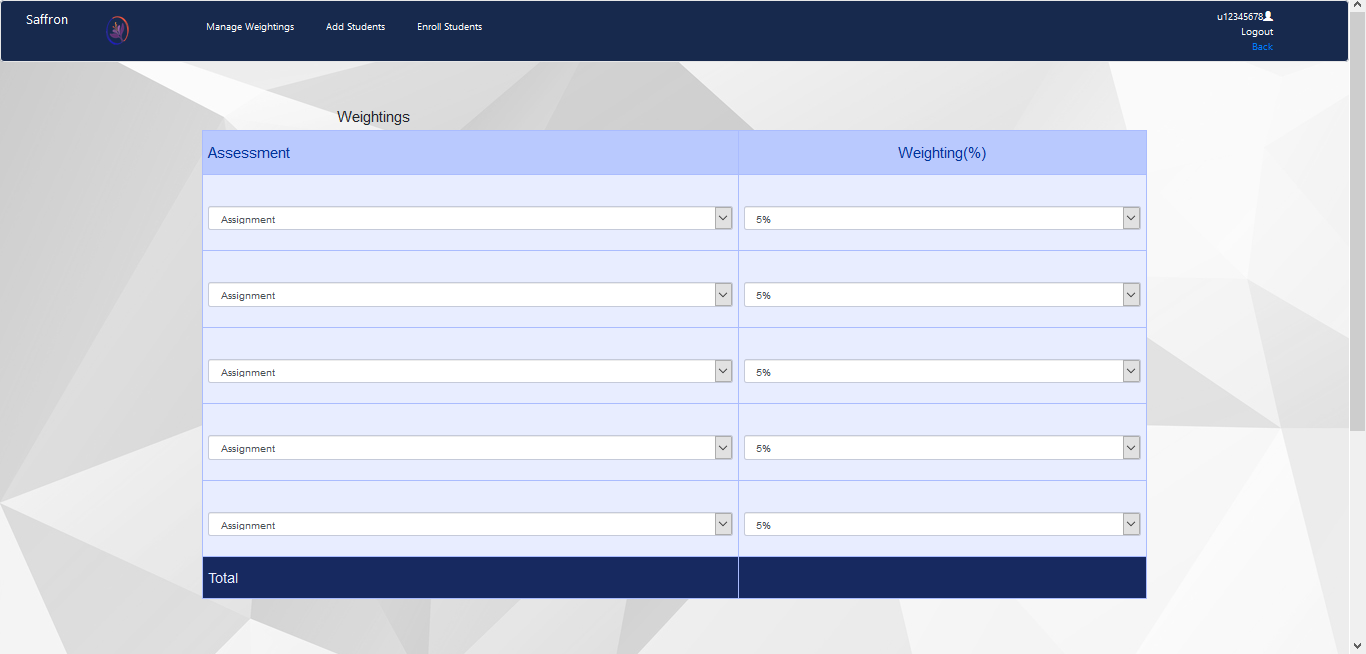
\includegraphics[width=1\textwidth]{../images/screens/weightings.PNG}\\[1.0cm]
        
        \subsection{Compose a query for an assessment}
        
        A student (user) can easily query their mark, given that the query time for that mark has not yet expired. The query structure is automatically generated, the user only has to provide a reason for their query and send it.
        
        %\includegraphics[width=1\textwidth]{../images/screens/student-query.PNG}\\[1.0cm]
        
        \subsection{View queries for assessments of a module}
        
        If a user has the correct permissions, they have the rights to view queries for all assessments of a specific module.
        
        %\includegraphics[width=1\textwidth]{../images/screens/admin-query.PNG}\\[1.0cm]
        
        \subsection{Add staff members with permissions}
        
        A user with the correct permissions, will be able to authorize other users.
        
        \subsection{Running an analysis on a CSV}
        
        Given the correct permissions, select a .csv file from the file dialog. Select either run student analysis or run module analysis. This will display a graph showing the relevant data. The blue line is the marks that have been obtained, and the red line is a trend line showing the general direction of your marks going forward. If the run line falls below the red line, it shows there is a danger of you failing and it should be quickly rectified.
        
        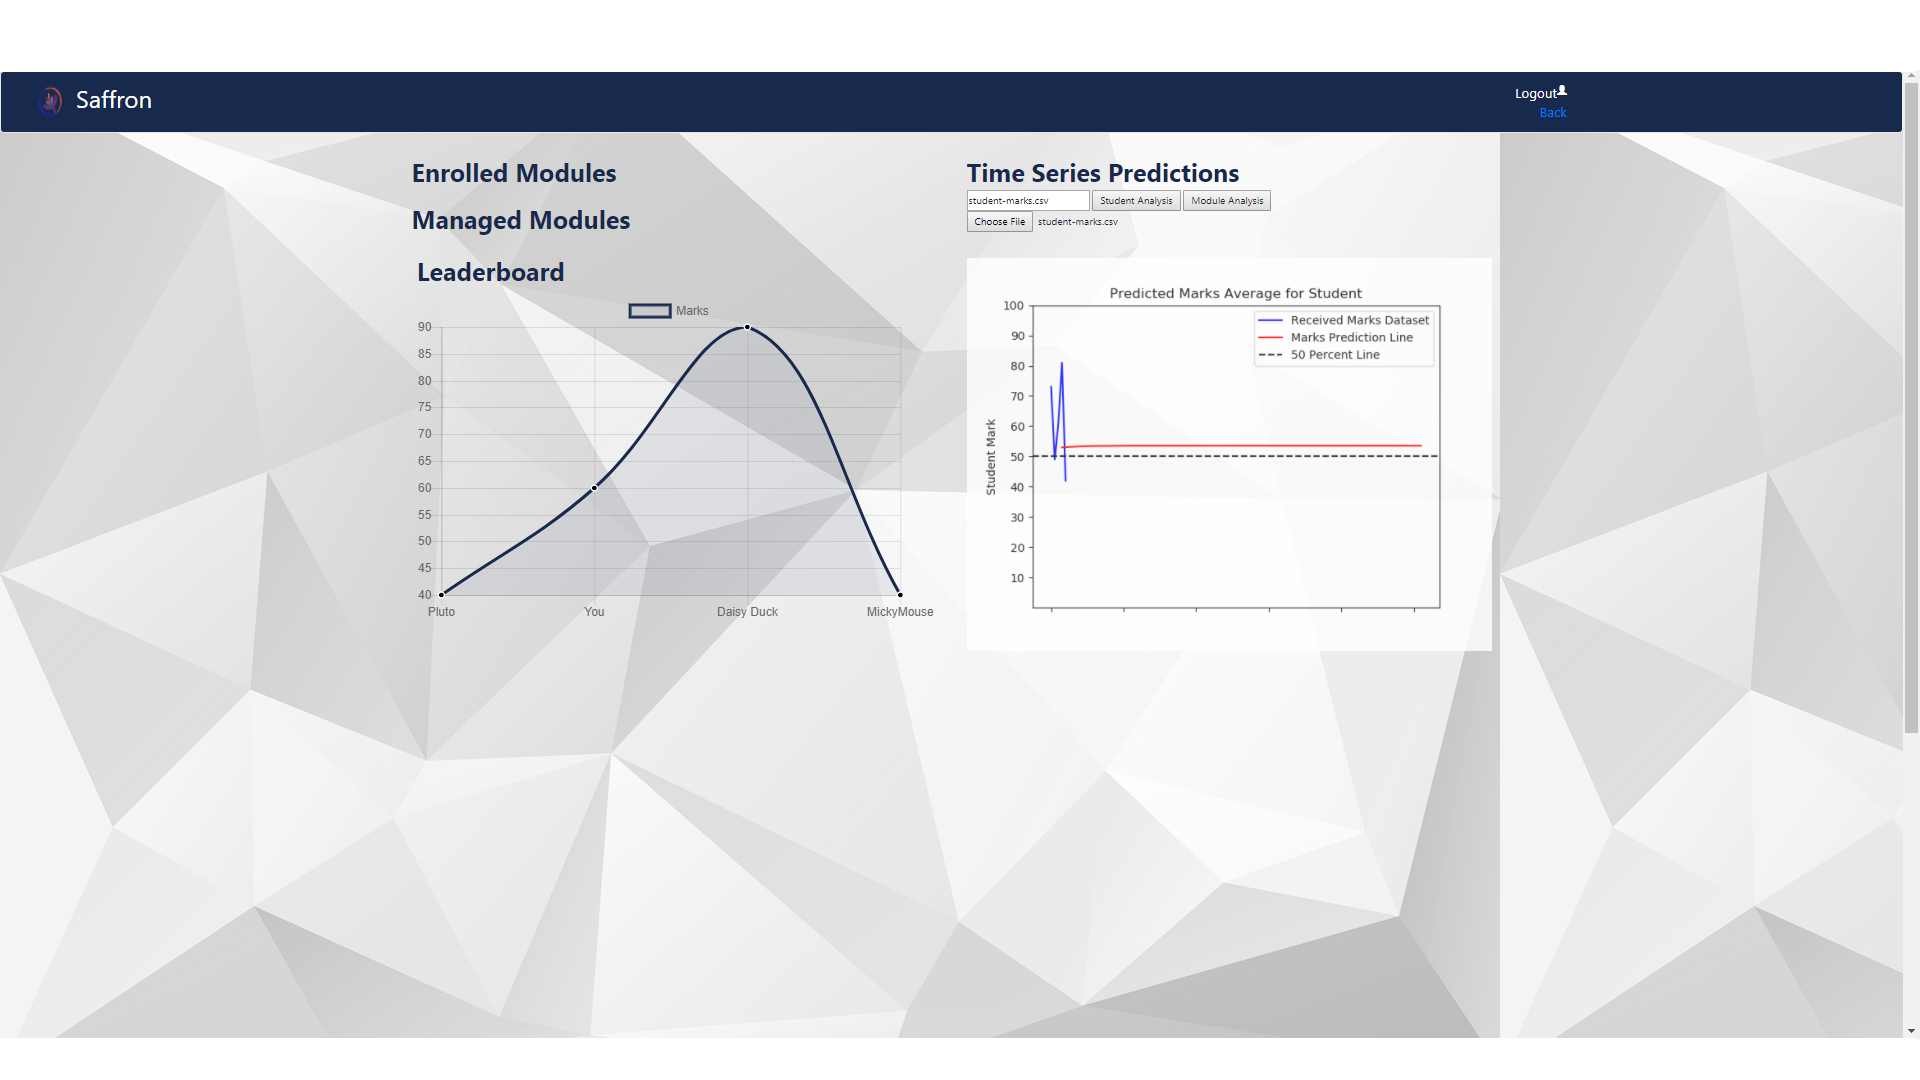
\includegraphics[width=1\textwidth]{../images/screens/student-analysis.PNG}\\[1.0cm]
        
    \pagebreak
     
    \section{Troubleshooting}
    
	    % Issues that are known to occur in the system and have not yet been solved
	    \subsection{Known system issues}
	    
	    At this time, no major issues are known.
	    
	    % Error messages that may occur in the system and what exactly they mean
	    \subsection{System error messages}
	    
	    \begin{itemize}
	    	\item \textbf{You are not authorized}
	    	\begin{itemize}
	    		\item The following error message means you do not have the required permissions to perform an action, and should contact a system administrator to obtain such permissions if required.
	    	\end{itemize}
	    \end{itemize}
	    
	    % Questions that commonly tend to come up regarding the system
	    \subsection{Frequently asked questions}
	    
	    \begin{itemize}
	    	\item \textbf{Why is the red line reaching 100 when that should be impossible?}
	    		\begin{itemize}
	    			\item The red line does not indicate an actual mark, but a trend in your marks. An average distribution of marks will generally create a straight line, a large improvement may show a huge spike to show increase in performance. If the red line does fall below the 50 mark, you are at risk of failing. If it is only below 50, it shows little to no chance of coming back.
	    		\end{itemize}
	    \end{itemize}
	 
	\pagebreak
	 
    \section{Appendixes}
    
    \section{Index}
    
    \pagebreak  

\end{document}
